%versi 3 (22-07-2020)
\chapter{Landasan Teori}
\label{chap:teori}
Pada bab ini berisikan penjelasan tentang teori-teori yang perlu diketahui sebelum pengembangan halaman web dilakukan. 

\section{\textit{Command-line Interface}}
\label{sec:CLI}
%jangan lupa tambahakan cite
\textit{Command-line interface}(CLI) merupakan sebuah antarmuka pengguna yang berbasis teks yang digunakan untuk menjalankan program, mengelola berkas-berkas pada komputer, dan dapat berinteraksi dengan komputer\footnote{https://www.techtarget.com/searchwindowsserver/definition/command-line-interface-CLI}.\textit{Command-line interface} juga disebut sebagai \textit{command-line user interfaces}, \textit{console user interfaces}, dan \textit{character user interfaces}. \textit{Command-line interface} menerima sebuah perintah yang diinput melalui keyboard perintah yang dipanggil oleh \textit{command prompt} yang dijalankan oleh komputer.

\textit{Command-line interface} langsung dapat berfungsi ketika sistem komputer dijalankan. \textit{Command-line interface} dapat terbuka di layar kosong dengan \textit{command prompt} lalu perintah-perintah dapat dimasukkan.   

\begin{figure}[H]
	\centering
	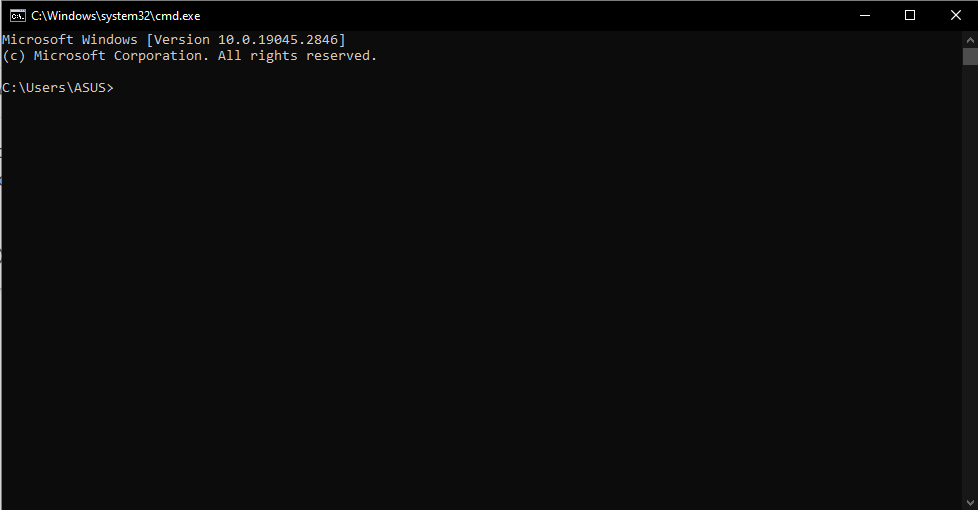
\includegraphics[width=0.8\textwidth]{Gambar/commandprompt.png}
	\caption{\textit{Command Prompt}}
	\label{fig:cmd}
\end{figure}

Jenis perintah-perintah dari \textit{Command-line interface} akan berisikan :

\begin{enumerate}
	\item Perintah-perintah dari sistem yang dikodekan sebagai bagian dari antarmuka sistem operasi
	\item Program yang dapat dijalankan ketika berhasil dipanggil,dan menjalankan aplikasi yang berbasis teks atau grafis.
	%tambahkan footnote untuk batch program
	\item \textit{batch program}\footnote{file teks yang berisi serangkaian perintah yang dimaksudkan untuk dieksekusi oleh \textit{command interpreter}}(\textit{batch files} atau \textit{shell script}) yang merupakan berkas teks berisikan urutan perintah-perintah. Ketika perintah berhasil dipanggil, \textit{batch program} akan menjalakan perintahnya yang mungkin berisikan sebuah perintah sistem dan program yang dapat dieksekusi.
\end{enumerate}
%tambahakan cite untuk scp referensi buku
Perintah \textit{Command-line interface} yang digunakan antaralain :
\subsection{SCP(\textit{Secure Copy Protocol})}
Salah satu perintah yang terdapat pada \textit{Command-line interface} yaitu SCP(\textit{secure copy}). SCP memiliki fungsi yang mirip seperti pada perintah \emph{cp}(\textit{copy}) yaitu untuk menyalin berkas\cite{william:19:linux}. Perbedaannya yang paling terlihat terletak pada sumber atau tujuan ke \textit{remote host}. Sebagai contoh, jika ingin menyalin sebuah dokumen dari \textit{local directory}(berkas dalam komputer) ke \textit{remote system}, atau dari \textit{working directory} ke \textit{local directory}. 

\begin{lstlisting}[language=Bash, caption=Pemanggilan SCP,label={code:callscp}]
	C:\Users\Asus>scp ssh i17086@10.100.69.101:Kota_Bandung.txt	
\end{lstlisting}

Kode program \ref{code:callscp} merupakan contoh penyalinan berkas Kota\textunderscore Bandung.txt. Berkas tersebut yang tersimpan didalam \textit{remote host} dan disalin ke \textit{local directory} pengguna.


\section{Hadoop Distributed File System}
\label{sec:hdfs}
%HDFS \textit{Hadoop Distributed File System} merupakan sistem file yang terdistribusi yang dapat diakses oleh pengguna untuk membaca(\textit{read}) dan menulis(\textit{write}) data. HDFS digunakan untuk sebagai tempat penyimpanan berkas-berkas yang berukuran besar pada \textit{Hadoop}.
HDFS (\textit{Hadoop Distributed File System}) merupakan sistem file terdisribusi yang berada pada penyimpanan server dan memiliki banyak kesamaan pada \textit{base storage system}. Sistem penyimpanan terdistribusi ini dapat menyimpan data dalam jumlah yang sangat besar melalui jaringan komputer dengan redudansi bawaan untuk melindungi data. HDFS dirancang untuk pemrosesan yang cepat dan toleran terhadap kesalahan, sehingga memungkinkan pengguna \textit{hardware} pada penyimanan tidak terkana biaya yang mahal.

HDFS memungkinkan para pengguna untuk menyimpan data kedalam file yang dibagi menjadi beberapa \textit{block}. Karena \textit{Hadoop} dirancang untuk bekerja dengan jumlah data yang besar, ukuran \textit{block} pada HDFS jauh lebih besar daripada yang digunakan oleh \textit{typical relational databases}. Dengan ukuran awal \textit{block} sebesar 128MB, dan dapat dikonfigurasi ukurannya mencapai 512MB.\cite{sam:16:hadoop}

HDFS memiliki 2 jenis \textit{node}, yaitu \textit{namenode} sebagai \textit{node master} dan \textit{datanode} sebagai \textit{node slave}. Kelebihan utama yang ditawarkan HDFS adalah \textit{scalability} dan \textit{availability} yang dicapai dikarenakan memiliki kemampuan replikasi data dan \textit{fault tolerance}.Dengan adanya kemampuan replikasi data/file, ketika ada kegagalan \textit{software }atau \textit{hardware}, HDFS akan melakukan replikasi ulang blok-blok data pada \textit{node} yang mengalami kegagalan.\cite{alex:14:hadoop}

Semua perintah HDFS dipanggil menggunakan \textit{script} \textit{bin/hdfs}. Penjalanan \textit{script} \textbf{"hdfs"} tanpa argumen akan mencetak deskripsi untuk semua perintah.\footnote{https://hadoop.apache.org/docs/stable/hadoop-project-dist/hadoop-hdfs/HDFSCommands.html}
\begin{lstlisting}[language=Bash, caption=Perintah HDFS CLI,label={code:hdfscli}]
	C:\Users\Asus>hdfs [SHELL_OPTION] COMMAND [GENERIC_OPTIONS] [COMMAND_OPTIONS]
\end{lstlisting}
Kode program \ref{code:hdfscli} merupakan pemanggilan perintah pada HDFS. Setiap opsi perintah memiliki fungsi untuk menajalankan \textit{script} pada CLI. Penjelasan tiap opsi dijelaskan pada tabel \ref{table:command_options}.  

\begin{table}[ht]
	\caption{Hadoop memiliki opsi parsing framework yang menjelaskan setiap fungsi kelasnya}
	\label{table:command_options}
	\resizebox{\columnwidth}{!}{%
		\begin{tabular}{|l|l|}
			\hline
			COMMAND\_OPTION          & Deskripsi                                                     \\ \hline
			SHELL\_OPTIONS           & kumpulan shell\_option yang umum                              \\ \hline
			GENERIC\_OPTIONS         & kumpulan generic\_option yang didukung oleh beberapa perintah \\ \hline
			COMMAND COMMAND\_OPTIONS & Bermacam perintah dengan opsi                                 \\ \hline
		\end{tabular}
	}
\end{table}


Penggunaan perintah HDFS yang digunakan antara lain :
\begin{enumerate}
	\item Penggunaan perintah \textbf{dfs}\\
	Perintah \textbf{dfs} digunakan untuk menjalankan(\textit{run}) perintah \textit{filesystem} yang didukung oleh \textit{Hadoop}. \textit{\textbf{[COMMAND\_OPTIONS]}} dapat dilihat pada \href{https://hadoop.apache.org/docs/stable/hadoop-project-dist/hadoop-common/FileSystemShell.html}{\textit{File System Guide}}. Contoh pemanggilan \textbf{dfs} seperti pemanggilan pada Gambar \ref{code:dfs}
	
	\begin{lstlisting}[language=Bash, caption=Perintah HDFS dfs,label={code:dfs}]
		C:\Users\Asus>hdfs dfs [COMMAND [COMAND_OPTIONS]]
	\end{lstlisting}
	
	\item Penggunaan perintah \textbf{get}\\
	Perintah \textbf{get} digunakan untuk menyalin file HDFS ke \textit{local system}.Gambar \ref{code:get} merupakan contoh yang menunjukkan cara penggunaan perintah \textbf{-get} untuk mengunduh file dari HDFS ke \textit{local file system}
	\begin{lstlisting}[language=Bash, caption=Perintah HDFS dfs -get untuk mengunduh file HDFS Kota\_Bandung.txt ke \textit{local system},label={code:get}]
		C:\Users\Asus>hdfs dfs -get /user/if18059/geodata/cropped/arcgis/16/Jawa_Barat/Kota_Bandung.txt .
	\end{lstlisting}
	\item Penggunaan perintah \textbf{-ls}\\
	Perintah \textbf{-ls} digunakan untuk menampilkan daftar isi \textit{directory} yang ditentukan oleh \textit{path} yang disediakan oleh pengguna. Gambar merupakan contoh yang menunjukkan cara penggunaan perintah \textbf{-ls} untuk melihat isi file HDFS.
	\begin{lstlisting}[language=Bash, caption=Perintah HDFS dfs -get untuk mengunduh file HDFS Kota\_Bandung.txt ke \textit{local system},label={code:ls}]
		C:\Users\Asus>hdfs dfs -ls /user/if18059/geodata/cropped/arcgis/16/Jawa_Barat
	\end{lstlisting}
\end{enumerate}



\section{\textit{Python}}
\label{sec:python}
%\textit{Python} Merupakan sebuah bahasa pemograman komputer yang dikembangkan khusus untuk membuat \textit{source code} yang mudah untuk dibaca. Bahasa pemograman \textit{pyhton} memiliki \textit{libary} yang lengkap sehingga memudahkan seorang pengembang untuk membuat sebuah aplikasi sesuai dengan keinginan dengan menggunakan \textit{source code} yang terlihat sederhana.
%cite
\textit{Python} adalah bahasa pemrograman yang memulai debutnya pada tahun 1991. \textit{Python} mencakup \textit{object-oriented programming} dan memperkenalkan \textit{syntax} yang membuat banyak \textit{operations} menjadi sangat ringkas dan elegan. Hal yang harus diperhatikan oleh \textit{programmers} baru mengenai \textit{Python} adalah pemakaian spasi(" ") sangat berpengaruh pada arti program yang dikembangkan. Pada proses pengembangan menggunakan bahasa \textit{Python} harus menggunakan \textit{text editor} yang dapat mengenali \textit{syntax}-nya agar memudahkan membuat program sesuai yang diinginkan.\cite{john:22:data}

Bahasa pemrograman \textit{Python} Merupakan sebuah bahasa pemograman komputer yang dikembangkan khusus untuk membuat \textit{source code} yang mudah untuk dibaca. \textit{Pyhton} memiliki \textit{library} yang lengkap sehingga memudahkan seorang \textit{programmer} untuk membuat sebuah aplikasi sesuai dengan keinginan dengan menggunakan \textit{source code} yang terlihat sederhana.

\subsection{\textit{Pillow (PIL Fork)}}
\label{subsec:python PIL}
\textit{Python Imaging Library} merupakan salah satu \textit{library} yang terdapat pada bahasa pemrograman \textit{Python}.PIL dapat menambahkan pemrosesan gambar ke bahasa pemrograman \textit{Python}.\textit{Library} ini menyediakan \textit{extensive file format}, representasi internal yang efisien, dan memiliki kemampuan yang baik dalam pemrosesan gambar. Pentingnya \textit{library} yang dirancang untuk dapat mengakses data yang disimpan dengan cepat dalam berbagai format piksel. Seharusnya memberikan dasar yang kuat sebagai alat pengolahan gambar\footnote{https://pillow.readthedocs.io/en/stable/handbook/overview.html}.
%cite dari website pillow fork doc

\textit{Python Imaging Library} sangat ideal untuk pengarsipan gambar dan aplikasi pemrosesan \textit{batch}. Penggunakan \textit{library }untuk membuat thumbnail, mengonversi antara format file, mencetak gambar, dll. Versi saat ini dapat mengidentifikasi dan membaca sejumlah besar format. Pembantuan dalam penulisan ini sengaja dibatasi dalam format pertukaran dan representasi yang paling umum digunakan.

\textit{Python Imaging Library} yang rilis saat ini mencakup antarmuka Tk \textit{PhotoImage} dan \textit{BitmapImage}, serta \textit{Windows DIB interface} yang dapat digunakan dengan \textit{PythonWin} dan berbagai mnacam \textit{toolkits} yang berbasis Windows. Banyak \textit{toolkits} GUI(\textit{Grapical User Interface}) lainnya yang dilengkapi dengan dukungan PIL. Untuk \textit{debugging}, ada juga metode \textit{show()} yang menyimpan gambar ke disk, dan memanggil utilitas tampilan eksternal.

\subsubsection{Penggunaan kelas\textit{Image}}
Dalam penggunaan \textit{Python Imaging Library} terdapat kelas yang paling penting yaitu kelas \textit{Image}, yang didefinisikan dalam modul dengan nama yang sama. Pembuat \textit{instance} dari kelas ini dengan beberapa cara; Baik dengan memuat gambar dari file, memproses gambar lain, atau membuat gambar dari awal. Memuat gambar dari file. 

\begin{enumerate}
	\item Penggunaan fungsi \textit{Image.open()}\\
	Berfungsi untuk membuka dan mengidentifikasi file gambar yang diberikan. Fungsi ini mengidentifikasi sebuah file, tetapi file tetap terbuka dan data gambar tidak terbaca sampai data file gambar tersebut diproses. Memiliki parameter \textbf{fp} merupakan nama file yang akan dibuka, \textbf{mode} memiliki argumen "r", dan \textit{\textbf{formats}} sebuah daftar format untuk memcoba memuat file. Parameter ini dapat digunakan untuk membatas format yang akan diperiksa. Dalam penggunaan fungsi dapat dilihat pada kode program \ref{code:openimage}.
	\begin{lstlisting}[language=Python, caption=Pemanggilan fungsi \textit{open()},label={code:openimage}]
		from PIL import Image
		
		im = image.open("hopper.ppm")
	\end{lstlisting}
	Jika pemanggilan fungsi berhasil, fungsi yang dipanggil akan mengembalikan sebuah objek \textit{Image}
	\item Penggunaan fungsi \textit{Image.new()}\\
	Berfungsi untuk membuat gambar baru dengan mede dan ukuran yang diberikan. Memiliki parameter \textbf{mode} untuk menentukan jenis dan kedalaman piksel dalam gambar seperti mode "L"(8-bit piksel,skala abu-abu), "RGB" (3x8-bit piksel,warna asli), "RBGA" (4x8-bit piksel, warna asli dengan \textit{transparacy mask}), dll. Parameter \textit{\textbf{size}} merupakan ukuran dari gambar baru, berisi ukuran horizontal dan vertikal dalam piksel. Parameter \textit{\textbf{color}} memberikan warna apa yang akan digunakan. Biasanya akan lansung diberikan warna hitam.
	\begin{lstlisting}[language=Python, caption=Pemanggilan fungsi \textit{new()},label={code:imagenew}]
		from PIL import Image
		
		im = image.new("hopper.ppm")
	\end{lstlisting}
	Jika pemanggilan fungsi pada gambar \ref{code:imagenew} berhasil, maka akan mengembalikan sebuah objek \textit{image}.
	\item Penggunaan fungsi \textit{Image.paste()}\\
	Berfungsi untuk menempelkan sebuah objek gambar ke objek gambar lain. Ukuran gambar yang ditempelkan harus sesuai dengan ukuran gambar. Memiliki parameter \textbf{im} yang merupakan sebuah objek image atau nilai piksel. Parameter \textit{\textbf{box}} 4-tupel opsional yang memberikan wilayah untuk ditempelkan. Jika 2-tupel digunakan sebagai gantinya, itu diperlakukan sebagai sudut kiri atas. Jika dihilangkan atau tidak ada, objek gambar yang ditempelkan ke sudut kiri atas. Parameter \textit{\textbf{mask}} merupakan sebuah optional \textit{mask} gambar.
	\begin{lstlisting}[language=Python, caption=Pemanggilan fungsi \textit{paste()},label={code:imagepaste}]
		from PIL import Image
		
		im = image.new("hopper.ppm")
		im1 = image.open()
		
		im.paste(im1,(256,256))
	\end{lstlisting}
	Jika fungsi pemanggilan pada gambar \ref{code:imagepaste} berhasil, akan mengembalikan sebuah objek \textit{Image} yang memuat gambar im1 yang ditempelkan pada gambar baru im.
	\item Penggunaan fungsi \textit{Image.save()}\\
	Berfungsi untuk menyimpan gambar dengan nama file yang diberikan. Jika tidak memiliki format yang ditentukan, maka format yang akan digunakan ditentukan dari ekstensi penamaan file, jika memungkinkan. memiliki beberapa parameter diantaranya adalah \textbf{fp} merupakan nama file yang akan digunakan memiliki tipe data string, parameter \textbf{format} merupakan format file yang akan digunakan pada file tersebut, dan \textbf{params} merupakan parameter tambahan untuk penulisan gambar.
\end{enumerate}


%\subsubsection{\textit{Reading and writing images}}
%\textit{Python Imaging Library} mendukung berbagai format file gambar. Pembacaan file dari disk,dapat digunakan fungsi \textit{open()} pada modul \textit{Image}. Juga tidak perlu mengetahui format file untuk membuka file. \textit{Library} secara otomatis menentukan format berdasarkan konten file. Penggunaan metode \textit{save()} (Gambar \ref{fig:saveimage}) dari kelas \textit{Image} untuk menyimpan file. Penamaan file sangat penting saat ingin melakukan pemyimpanan. Kecuali format pada penyimpanan telah ditentukan, \textit{library} dapat menggunakan ekstensi \textit{filename} dalam menemukan format penyimpanan file mana yang akan digunakan.
%\begin{figure}[H]
%	\centering
%	%	\captionsetup{width=.9\linewidth}
%	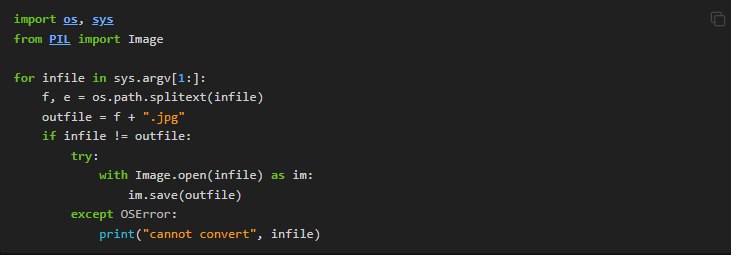
\includegraphics[width=0.8\textwidth]{Gambar/functionsave.png}
%	\caption{Mengkonversikan File kedalam bentuk JPEG}
%	\label{fig:saveimage}
%\end{figure}

%\subsubsection{\textit{Pasting and merging images}}
%Metode \textit{paste} merupakan metode yang paling populer dan nyaman untuk menempelkan gambar pada gambar lain. Penggunaan \textit{paste} diterapkan ke gambar yang ada dan argumen pertamanya adalah gambar yang ditempelkan.
%Argumen kedua adalah sebuah kotak. Kotak ini bisa berupa tupel 2 elemen atau 4 elemen. Jika Anda menggunakan 2 elemen, itu akan menentukan di mana sudut kiri atas gambar yang ditempel dimulai. Jika Anda menggunakan 4 elemen maka Anda akan mendefinisikan semua 4 sudut gambar yang ditempelkan relatif terhadap gambar dasar.

\section{\textit{Base64}}
\label{sec:base64}

Base64 merupakan sebuah algoritma yang digunakan untuk mengubah tipe data \textit{bytes} menjadi tipe data yang dapat dilihat(dan sebaliknya). Skema pengkodean biner ke teks pada Base64 sebagai persyaratan untuk mengirim tipe data \textit{bytes} melalui jaringan komunikasi yang tidak mengizinkan tipe data biner tetapi hanya tipe data berbasis teks.Data teks yang dihasilkan terdiri dari berbagai karakter yang terdapat pada standar ASCII. Penggunaan kata Base64 berasal dari jumlah karakter ASCII yang digunakan. 64 karakter yang digunakan antara lain adalah 26 karakter a-z \textit{lowercase}, 26 karakter A-Z \textit{uppercase}, ditambah dengan 2 karakter tambahan yaitu karakter tambah ”+” dan karakter garis miring ”/”. Base64 juga sebenarnya memiliki karakter ke 65 yaitu karakter sama dengan ”=” yang digunakan sebagai \textit{padding}. Karakter sama dengan (”=”) digunakan pada segmen terakhir data biner yang tidak memiliki total 6 \textit{bit}. Keseluruhan karakter yang digunakan pada Base64 disebut juga tabel enkoding Base64.

Base64 bekerja dengan cara memotong data biner menjadi segmen-segmen berukuran 6 \textit{bit}. Base64 hanya menggunakan 6 \textit{bit} untuk bisa memenuhi seluruh karakter yang digunakan (26 = 64). Masing-masing segmen tersebut kemudian dibaca ke dalam tipe desimal lalu dikonversi ke karakter ASCII. Sebagai contoh konversi data yang berisi 3 buah \textit{byte} yaitu 155, 162, dan 233. Tipe data \textit{byte} diubah menjadi data biner dan diambung menjadi satu yaitu 100110111010001011101001. Kemudian data biner dipotong menjadi segmen yang berisi 6 \textit{bit} menjadi 100110, 111010, 001011, 101001. Masing-masing data dikonversi menjadi desimal , 58, 11, 4yaitu 381. Terakhir data dikonversikan ke karakter ASCII yang berada pada tabel enkoding Base64 menjadi m6Lp. Cara yang sama namun terbalik prosesnya digunakan untuk mendeskripsi data dari Base64 kembali ke tipe data \textit{byte}.\cite{juan:22:pengumpulan}
%cite skripsi juan

\section{Framework Laravel}
\label{sec:framework}
\textit{Framework} adalah kerangka kerja yang digunakan oleh developer untuk memudahkan pembangunan aplikasi web yang dapat berupa sekumpulan \textit{libary} yang berisi fungsi, \textit{tools}, ataupun \textit{class-class}, dan digunakan sebagai kerangka dalam pembangunan aplikasi web. Umumnya didlama framwork telah menyediakan solusi untuk dapat mengakses \textit{database}, \textit{authentication}, \textit{templating}, \textit{controls}, dan fungsi-fungsi lainnya/ Dalam penggunaan \textit{framework} diharapkan dapat membuat pengembangan aplikasi menajdi rapi dan bersih, memiliki struktur yang optimal, dan \textit{reusable}. 

Laravel adalah \textit{framework} aplikasi web dengan sintaks yang ekspresif dan elegan. Laravel adalah \textit{framework} berbasis PHP yang sifatnya \textit{open source}, dan menggunakan konsep \textit{model-view – controller}. Laravel berada di bawah lisesni MIT \textit{License} dengan menggunakan Github sebagai tempat berbagi code menjalankannya. Laravel berlisensi \textit{open source} yang artinya bebas digunakan tanpa harus melakukan pembayaran. Alamat website remis dari \textit{framework} Laravel adalah \url{https://laravel.com}. Kelebihan laravel adalah sebagai berikut:

\begin{itemize}
	\item Progresif \textit{Framework} \\
	Progresif yang dimaksud adalah framework ini dapat bertumbuh bersama developer. Yang artinya dapat diikuti oleh developer baru maupun developer senior dikarenakan terdapat dokumentasi, panduan, dan tutorial video laravel yang dapat membantu membangun perangkat lunak.
	\item Komunitas \textit{Framework} \\
	Pada laravel terdapat banyak sekali \textit{packages} terbaik dalam ekosistem PHP. selain itu, ribuan pengembang berbakat dari seluruh dunia telah berkontribusi pada \textit{framework} ini.
	\item Berskala \textit{Framework} \\
	Laravel memberikan dukungan sistem cache yang terdistribusi dengan cepat. Faktanya laravel dapat menangani ratusan juta \textit{request} setiap bulan.
\end{itemize}

Dalam penggunaan laravel memiliki beberapa kekurangan salah satunya yaitu ukuran file yang cukup besar. Di dalam laravel terdapat file yang sifatnya default seperti vendor. File tersebut tidak boleh dihapus sembarangan sehingga ukuran website yang dibuat berukuran cukup besar. Selain itu, dibutuhkan koneksi internet untuk instalasi dan mengunduh \textit{library} laravel, dan PHP minimal versi 5.4 untuk menjalankannya. Berikut adalah dasar-dasar laravel:
\begin{enumerate}
	\item Artisan \\
	Artisan adalah command line atau perintah yang dijalankan melalui terminal dan disediakan beberapa perintah perintah yang dapat digunakan selama melakukan pengembangan dan pembuatan aplikasi. Salah satu fungsi dari php artisan yaitu “php artisan serve”. Php artisan serve berfungsi untuk membuka website yang telah dibuat tanpa menggunakan web server lokal. Gambar \ref{fig:artisan} merupakan contoh salah satu penggunaan artisan dalam laravel.
	
	\begin{figure}[H]
		\centering
		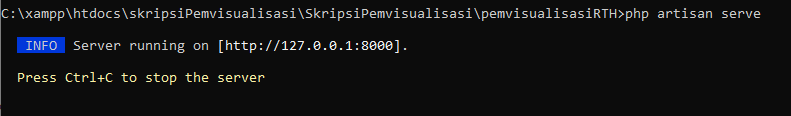
\includegraphics[width=0.8\textwidth]{Gambar/artisan.png}
		\caption{PHP Artisan Laravel}
		\label{fig:artisan}
	\end{figure}
	\item \textit{Controller} \\
	\textit{Controller} merupakan suatu proses yang bertujuan untuk mengambil data, menambahkan data, menghapus data, atau mengubah data untuk ditampilkan dalam halaman. Cara membuat \textit{controller} adalah dengan menggunakan \textit{command line} dengan memasukkan "php artisan make controller <<nama\_controller>>". File \textit{controller} nantinya akan otomatis terbuat dan sudah masuk ke folder \textit{controller}.
	
	
	\item \textit{Routing} \\
	\textit{Routing} merupakan suatu proses yang dapat memindahkan tampilan halaman ke halaman lain. Dengan menggunakan \textit{routing}, pengguna dapat menentukan halaman yang ingin dikunjungi. Pengaturan \textit{routing} di laravel terletak pada file \textit{web.php}.
	
	
	\item \textit{Blade View} \\
	\textit{Blade} adalah \textit{template engine}. Pada dasarnya \textit{Blade} adalah \textit{view} namun dengan menggunakan \textit{Blade} akan mempermudah untuk mengatur tampilan \textit{website} dan menampilkan data. Cara untuk membuat file \textit{view} menjadi file \textit{Blade} adalah dengan menambahkan ekstensi .blade.php pada file \textit{view}. Dan cara unutk memanggil file \textit{Blade} sama dengan cara untuk memanggil file \textit{view} biasa.
\end{enumerate}	

Setelah melakukan penginstallan Laravel akan terlihat direktori yang berisi aplikasi Laravel dasar. File dan direktori yang terdapat sebagai berikut:\cite{matt:19:laravel}
%referensi dari Stauffer, Matt - Laravel_ a Framework for Building Modern PHP Apps-O'Reilly Media, Incorporated (2019)
	\begin{itemize}
		\item[] \textbf{app/}
		\item[] \textbf{bootstrap/}
		\item[] \textbf{config/}
		\item[] \textbf{public/}
		\item[] \textbf{resources/}
		\item[] \textbf{routes/}
		\item[] \textbf{storage/}
		\item[] \textbf{tests/}
		\item[] \textbf{vendor/}
		\item[] .editorconfig
		\item[] .env
		\item[] .env.example
		\item[] .gitattributes
		\item[] .gitignore
		\item[] artisan
		\item[] composer.json
		\item[] composer.lock
		\item[] package.json
		\item[] phpunit.xml
		\item[] readme.md
		\item[] server.php
		\item[] webpack.mix.js
	\end{itemize}
	
Direktori utama (\textit{root directory}) mengandung folder-folder berikut secara \textit{default}:
	\begin{itemize}
		\item  \textit{app}\\
		Berisikan sebagian besar aplikasi saat dijalankan. \textit{Model}, \textit{controller}, \textit{commands}, dan kode domain PHP yang dibuat semuanya akan berada di direktori ini.
		\item  \textit{bootsrap} \\
		Berisi file-file yang digunakan oleh \textit{framework} Laravel saat setiap kali dijalankan.
		\item  \textit{config} \\
		Berisikan semua file konifgurasi aplikasi.
		\item  \textit{database} \\
		Berisi file \textit{databse migration} dan \textit{seeds}.
		\item  \textit{public} \\
		Direktori yang ditunjuk oleh server ketika menjalankan aplikasi web. Berisi file index.php, yang merupakan \textit{entry point} untuk menangani semua \textit{request} yang masuk ke aplikasi. Didalam folder ini dapat menyumpan beberapa aset dari aplikasi seperti gambar, \textit{JavaScript}, dan \textit{CSS}.
		\item  \textit{resource }\\
		Berisi file \textit{view} dari aplikasi yang dibuat. Didalam folder ini juga terdapat file \textit{language} yang digunakan aplikasi.
		\item  \textit{routes} \\
		Berisi file yang digunakan untuk mendefinisikan semua \textit{route} ke aplikasi. Secara \textit{default} ada tiga file \textit{route} yang disediakan oelh Laravel yaitu api.php, console.php, dan web.php.
		\item  \textit{storage} \\
		Berisi \textit{template Blade} yang dikompilasi, file \textit{session}, file \textit{cache}, dan file lainnya yang dihasilkan secara otomatis oleh Laravel.
		\item  \textit{tests} \\
		Berisi semua file \textit{test} yang dibuat untuk aplikasi.
		\item  \textit{vendor} \\
		Berisikan tempat \textit{Composer} menginstal dependensinya. Direktori ini akan diabaikan oleh Git, karena \textit{Composer} diharapkan dapat berjalan sebagai bagian dari proses implementasi pada server-server jarak jauh.
	\end{itemize}
Direktori utama juga berisi file-file berikut:
	\begin{itemize}
		\item .\textit{editorconfig} \\
		Memberikan instruksi kepada IDE/editor teks  tentang standar penulisan kode Laravel (seperti, ukuran indentasi, set karakter, dan apakah harus memotong \textit{whitespace} di ujung baris).
		\item \textit{.env }dan \textit{.env.example} \\
		Menentukan variabel-variabel lingkungan (variabel yang diharapkan berbeda di setiap lingkungan dan karena itu tidak dimasukkan ke dalam \textit{version control}). \textit{.env.example} adalah template yang setiap lingkungan harusnya menduplikasi untuk membuat file \textit{.env}-nya sendiri, yang akan diabaikan oleh Git.
		\item \textit{.gitattributes} dan \textit{.gitignore} \\
		Berisikan file-file untuk pengkonfigurasian Git.
		\item artisan \\
		Berisikan file untuk menajalakan perintah-perintah artisan dari \textit{command-line}.
		\item composer.json dan composer.lock \\
		Berisikan file konfigurasi untuk \textit{Composer}. \textit{composer.json} dapat diedit oleh pengguna sedangkan \textit{composer.lock} tidak dapat diedit. File-file ini berisi informasi dasar tentang proyek dan juga mendefinisikan dependensi dari PHP.
		\item package.json \\
		File yang berisikan sama seperti \textit{composer.json}, tetapi untuk aset \textit{front-end} dan dependensi dari sistem pembangunan. File ini juga memberi instruksi kepada NPM tentang dependensi berbasis \textit{JavaScript} yang harus diunduh.
		\item phpunit.xml \\
		Berisikan file konfigurasi untuk \textit{PHPUnit} merupakan alat yang digunakan Laravel secara \textit{default} untuk pengujian.
		\item readme.md \\
		Sebuah file \textit{Markdown} yang memberikan pengenalan dasar tentang Laravel. File ini tidak dapat dilihat jika menggunakan instalator dari Laravel.
		\item server.php \\
		Berisikan sebuah server cadangan yang mencoba untuk memungkinkan server yang kurang mampu agar tetap dapat melihat \textit{preview} aplikasi Laravel.
		\item webpack.mix.js \\
		File konfigurasi yasng bersifat optional untuk \textit{Mix}. Jika menggunakan Elixir, maka akan melihat \textit{gulpfile.js} sebagai gantinya. File-file ini digunakan untuk memberikan instruksi kepada sistem pembangunan tentang cara mengkompilasi dan memproses aset \textit{front-end }aplikasi Laravel.
	\end{itemize}



